\documentclass[11pt, oneside]{article}

\pdfoutput=1

\RequirePackage[utf8]{inputenc}
\RequirePackage[T1]{fontenc}
\RequirePackage{xcolor,graphicx}
\RequirePackage{hyperref}
\hypersetup{%
  colorlinks=true,
  breaklinks=true,
  linkcolor=red,
  anchorcolor=black,
  citecolor=brown,
  filecolor=blue,
  menucolor=red,
  urlcolor=red,
}
\RequirePackage[authoryear]{natbib}
\RequirePackage{xr}
\RequirePackage{mathtools, amsfonts, amssymb,amsthm}
\mathtoolsset{showonlyrefs}
\RequirePackage{enumerate}
\RequirePackage{comment}
\RequirePackage{ifthen}
\RequirePackage{enumerate}
\RequirePackage{comment}
\RequirePackage{subcaption}
\RequirePackage{siunitx}
\RequirePackage[ruled,vlined]{algorithm2e}

\externaldocument{ms}


\setlength{\textwidth}{16cm}
\setlength{\textheight}{22cm}
\setlength{\hoffset}{-1.4cm}
\topmargin -1cm 



%%%%%%%%%%%%%%%%%%%%%%%%%%%%%%%%%%%%%%%%%%%%%%%%%%%%%%%%%
%%%%%%%%%%% JDT:  Annotation Code %%%%%%%%%%%%%%%%%%%%%%%%%%%%%%%%%%
%%%%%%%%%%%%%%%%%%%%%%%%%%%%%%%%%%%%%%%%%%%%%%%%%%%%%%%%%

\RequirePackage{color}
\RequirePackage[normalem]{ulem}

 % Uncomment to display with annotation; comment out otherwise
\newcommand{\add}[1]{\textcolor{blue}{#1}}
\newcommand{\delete}[1]{\textcolor{red}{\sout{#1}}}
\newcommand{\edit}[2]{\textcolor{red}{\sout{#1}} \textcolor{blue}{#2}}
\newcommand{\mnote}[1]{\marginpar{\textcolor{green}{\textbf{#1}}}}


% -------------
% Some commands
% -------------

% Environment
\newcounter{rem}
\newtheorem{remark}[rem]{Remark}

\newcounter{th}
\newtheorem{theorem}[th]{Theorem}

\newcounter{lm}
\newtheorem{lemma}[lm]{Lemma}

\newcounter{scenario}[section]
\newenvironment{scenario}[1][]{\refstepcounter{scenario}\par\medskip
   \noindent \textbf{Scenario~\thescenario. #1} \rmfamily}{\medskip}

\newenvironment{results}[1][]{\noindent \textbf{#1} \rmfamily}{\medskip}

\providecommand{\keywords}[1]{\textbf{\textit{Keywords---}} #1}

% Stats
\newcommand{\EE}{\mathbb{E}} % Expectation
\newcommand{\RR}{\mathbb{R}} % R
\newcommand{\NN}{\mathbb{N}} % N
\newcommand{\XX}{\mathcal{X}} % set X
\newcommand{\dd}{{\rm d}}

% Spaces
\newcommand{\TT}[1]{\mathcal{T}_{#1}} % Domain definition space
\newcommand{\sLp}[1]{\mathcal{L}^{2}\left(#1\right)} % L^p space
\newcommand{\HH}{\mathcal{H}} % Product of L^p space
\newcommand{\GG}{\mathcal{G}} % (L^p)^N space

% Inner product and norm
\newcommand{\pointt}{\mathbf{t}} % Indexed of multivariate curves
\newcommand{\points}{\mathbf{s}} % Indexed of multivariate curves
\newcommand{\inLp}[2]{\left\langle#1, #2\right\rangle} % Inner product in Lp
\newcommand{\inR}[2]{\left(#1, #2\right)}
\newcommand{\inRM}[2]{\left(#1, #2\right)_{\mathbf{M}}}
\newcommand{\normLp}[1]{\left|\!\left|#1\right|\!\right|} % Norm in Lp
\newcommand{\normR}[1]{\left(\!\left(#1\right)\!\right)} %
\newcommand{\normRM}[1]{\left(\!\left(#1\right)\!\right)_{\mathbf{M}}} %
\newcommand{\inH}[2]{\langle\!\langle#1, #2\rangle\!\rangle}
\newcommand{\inHw}[2]{\langle\!\langle#1, #2\rangle\!\rangle_w}
\newcommand{\inHG}[2]{\langle\!\langle#1, #2\rangle\!\rangle_\Gamma}
\newcommand{\normH}[1]{\left|\!\left|\!\left|#1\right|\!\right|\!\right|}
\newcommand{\normHG}[1]{\left|\!\left|\!\left|#1\right|\!\right|\!\right|_\Gamma}

% Data/Process related
\newcommand{\Xnp}{X_n^{(p)}} % Observation n, feature p
\newcommand{\Xnq}{X_n^{(q)}} % Observation n, feature q
\newcommand{\hatXnp}{\widehat{X}_n^{(p)}} % Reconstruction
\newcommand{\Xp}[1]{X^{(#1)}} % Feature p
\newcommand{\hatXp}[1]{\widehat{X}^{(#1)}} % Reconstruction, Feature p
\newcommand{\mup}[1]{\mu^{(#1)}} % Feature p
\newcommand{\hatmup}[1]{\widehat{\mu}^{(#1)}} % Reconstruction, Feature p
\newcommand{\fp}{f^{(p)}} 
\newcommand{\gp}{g^{(p)}}

% Geometric related
\newcommand{\pobs}[1]{\mathrm{#1}} % Point related to observations
\newcommand{\CN}{\mathcal{C}_{\!N}} % Cloud of features
\newcommand{\Gmu}{\pobs{G}_{\!\mu}} % Centre of gravity of C_N
\newcommand{\OH}{\pobs{O}_{\!\mathcal{H}}} % Centre of H

\newcommand{\pfea}[1]{\mathsf{#1}} % Point related to features
\newcommand{\CP}{\mathcal{C}_{\!P}} % Cloud of observations
\newcommand{\Gfea}{\pfea{G}_{\!\mu}} % Centre of gravity of C_P
\newcommand{\OG}{\pfea{O}_{\!\RR}} % Centre of H

% Declaration of math operator
\DeclareMathOperator{\Var}{Var}
\DeclareMathOperator{\Cov}{Cov}
\DeclareMathOperator*{\argmax}{arg\,max}
\DeclareMathOperator{\bigO}{\mathcal{O}}

% Function subset restriction  
\newcommand\restr[2]{{ %
  \left.\kern-\nulldelimiterspace  %
  #1  %
  \vphantom{\big|}  %
  \right|_{#2}  %
}}
% -------------

\title{Supplementary material for ``On the use of the Gram matrix for multivariate functional principal components analysis''}

\author{%
Steven Golovkine\thanks{MACSI, Department of Mathematics and Statistics, University of Limerick, Ireland \href{mailto:steven.golovkine@ul.ie}{steven.golovkine@ul.ie}}
\and
Edward Gunning\thanks{Department of Biostatistics and Epidemiology, University of Pennsylvania, USA \href{mailto:edward.gunning@pennmedicine.upenn.edu}{edward.gunning@pennmedicine.upenn.edu}}
\and
Andrew J. Simpkin\thanks{School of Mathematical and Statistical Sciences, University of Galway, Ireland \href{mailto:andrew.simpkin@nuigalway.ie}{andrew.simpkin@nuigalway.ie}}
\and
Norma Bargary\thanks{MACSI, Department of Mathematics and Statistics, University of Limerick, Ireland \href{mailto:norma.bargary@ul.ie}{norma.bargary@ul.ie}}
}
\date{\today}

\begin{document}

\maketitle

In this Supplementary Material, we provide insights for when the data are already decomposed in a basis, e.g. Fourier or polynomials. In particular, we explain how to perform MFPCA as described in Section~\ref{sec:functional_principal_components_analysis} in the main text.

\renewcommand{\theequation}{SM.\arabic{equation}}


\section{Basis decomposition} % (fold)
\label{sub:basis_decomposition}


In many practical situations, functional data are noisy and only observed at specific time points. To extract the underlying functional features of the data, smoothing and interpolation techniques are commonly employed. These techniques involve approximating the true underlying function generating the data by a finite-dimensional set of basis functions. Assume that for each feature $p = 1, \dots, P$, there exists a set of basis of functions $\Psi^{(p)} = \{\psi_k^{(p)}\}_{1 \leq k \leq K_p}$ such that each feature of each curve $n = 1, \dots, N$ can be expanded using the basis:
\begin{equation}\label{eq:curve_basis_expansion}
\Xnp(t_p) = \sum_{k = 1}^{K_p} c^{(p)}_{nk}\psi_k^{(p)}(t_p), \quad t_p \in \TT{p},
\end{equation}
where $\{c^{(p)}_{nk}\}_{1 \leq k \leq K_p}$ is a set of coefficients for feature $p$ of observation $n$. We denote by $\overline{c}_k^{(p)} = \sum_{n = 1}^N \pi_n c^{(p)}_{nk}$ the mean coefficient of feature $p$ corresponding to the $k$th basis function.
The $p$th feature of the mean function can be then expanded in the same basis as:
\begin{equation}
    \hatmup{p}(t_p) = \sum_{k = 1}^{K_p} \overline{c}_k^{(p)}\psi_k^{(p)}(t_p), \quad t_p \in \TT{p}.
\end{equation}
Similarly, the covariance function of the $p$th and $q$th features is given by:
\begin{equation}
    \widehat{C}_{p,q}(s_p, t_q) = \sum_{k = 1}^{K_p} \sum_{l = 1}^{K_q} \left(\sum_{n = 1}^N \pi_n c^{(p)}_{nk}c^{(q)}_{nl} - \overline{c}_k^{(p)}\overline{c}_l^{(q)}\right)\psi_k^{(p)}(s_p)\psi_l^{(q)}(t_q), \quad s_p \in \TT{p},\quad t_q \in \TT{q}.
\end{equation}
These formulas can be written in matrix form as follows. For $\pointt \in \TT{}$, we have that $X(\pointt) = \mathbf{C}\Psi(\pointt)$ where $X(\pointt)$ is a $N \times P$ matrix with entries $\Xnp(t_p),~t_p \in \TT{p},~1 \leq p \leq P,~1 \leq n \leq N$,
\begin{equation}
    \mathbf{C} = \begin{pmatrix}
            \mathbf{C}^{(1)} & \cdots & \mathbf{C}^{(P)} \\
        \end{pmatrix}, \quad \text{and}\quad
    \Psi(\pointt) = \text{diag}\{\Psi^{(1)}(t_1), \dots, \Psi^{(P)}(t_P)\},
\end{equation}
where
\begin{equation}
\mathbf{C}^{(p)} = \begin{pmatrix}
    c^{(p)}_{11} & \cdots & c^{(p)}_{1K_p} \\
    \vdots & \ddots & \vdots \\
    c^{(p)}_{N1} & \cdots & c^{(p)}_{NK_p}
\end{pmatrix} \\
\quad \text{and}\quad
\Psi^{(p)}(t_p) = \begin{pmatrix}
    \psi_1^{(p)}(t_p) \\
    \vdots \\
    \psi_{K_p}^{(p)}(t_p)
\end{pmatrix}.
\end{equation}
Using the basis expansion and denoting $\Pi^\top = (\pi_1, \dots, \pi_N)$, the mean and covariance functions are given by
\begin{equation}
    \widehat{\mu}(\pointt) = \Psi(\pointt)^\top \mathbf{C}^\top\Pi \quad\text{and}\quad \widehat{C}(\points, \pointt) = \Psi(\points)^\top \mathbf{C}^\top \left(\text{diag}\{
        \pi_1, \dots, \pi_N\} - \Pi\Pi^\top\right)\mathbf{C} \Psi(\pointt).
\end{equation}
Finally, we denote by $\mathbf{W}$ the matrix of inner products of the functions in the basis $\Psi$. The matrix $\mathbf{W}$ is a block-diagonal matrix such that $\mathbf{W} = \text{blockdiag}\{\mathbf{W}^{(1)}, \dots, \mathbf{W}^{(P)}\}$ where each entry is given by
\begin{equation}
    \mathbf{W}_{k, l}^{(p)} = \inLp{\psi_k^{(p)}}{\psi_l^{(p)}}, \quad 1 \leq k, l \leq K_p, \quad 1 \leq p \leq P.
\end{equation}
We remark that, if the basis $\Psi$ is an orthonormal basis, the matrix $\mathbf{W}$ is equal to the identity matrix of size $\sum_{p = 1}^P K_p$.
Using the expansion of the data into the basis of functions $\Psi$, the inner-product matrix $\mathbf{M}$ is written 
\begin{equation}\label{eq:gram_matrix_basis}
    \mathbf{M} = \text{diag}\{
        \sqrt{\pi_1}, \dots, \sqrt{\pi_N}\}\left(\mathrm{I}_{\!N} - \mathbf{1}_{\!N}\Pi^\top\right) \mathbf{C} \mathbf{W} \mathbf{C}^\top \left(\mathrm{I}_{\!N} - \Pi\mathbf{1}_{\!N}^\top\right)\text{diag}\{
        \sqrt{\pi_1}, \dots, \sqrt{\pi_N}\}
\end{equation}
where $\mathrm{I}_{\!N}$ is the identity matrix of size $N$ and $\mathbf{1}_{\!N}$ is a vector of $1$ of length $N$.


% subsection basis_decomposition (end)


\section{MFPCA with a basis expansion} % (fold)
\label{sub:with_a_basis_expansion}

In this section, we assume that the observations are expanded into a basis of functions, as explained in Section~\ref{sub:basis_decomposition}. Using the expansion of the data into the basis of function $\Psi$ and $\mathbf{W}$, the matrix of inner products of the functions in the basis $\Psi$, we write \eqref{eq:gram_matrix_basis} as
\begin{equation}
    \mathbf{M} = \left(\text{diag}\{
        \sqrt{\pi_1}, \dots, \sqrt{\pi_N}\}\left(\mathrm{I}_{\!N} - \mathbf{1}_{\!N}\Pi^\top\right) \mathbf{C}\mathbf{W}^{1/2}\right)\left(\text{diag}\{
        \sqrt{\pi_1}, \dots, \sqrt{\pi_N}\}\left(\mathrm{I}_{\!N} - \mathbf{1}_{\!N}\Pi^\top\right) \mathbf{C}\mathbf{W}^{1/2}\right)^\top.
\end{equation}
We note
\begin{equation}
    \mathbf{A} = \text{diag}\{\sqrt{\pi_1}, \dots, \sqrt{\pi_N}\}\left(\mathrm{I}_{\!N} - \mathbf{1}_{\!N}\Pi^\top\right) \mathbf{C}\mathbf{W}^{1/2},
\end{equation}
such that $\mathbf{M} = \mathbf{A}\mathbf{A}^\top$.
We also assume that $\phi_1, \phi_2, \dots$ the eigenfunctions of the covariance operator $\Gamma$ have a decomposition into the basis $\Psi$
\begin{equation}
    \phi_k(\cdot) = 
        \begin{pmatrix} 
            \phi_k^{(1)}(\cdot) \\
            \vdots \\
            \phi_k^{(P)}(\cdot)
        \end{pmatrix} = 
        \begin{pmatrix} 
            \psi^{(1) \top}(\cdot) b_{1k} \\
            \vdots \\
            \psi^{(P) \top}(\cdot) b_{Pk}
        \end{pmatrix}, \quad\text{where}\quad
        b_{pk} = \left(b_{p k 1}, \dots, b_{p k K_p} \right)^\top.
\end{equation}
We have, for $p = 1, \dots, P$,
\begin{align*}
    \left(\Gamma \phi_k\right)^{(p)}(\cdot) &= \sum_{q = 1}^P \int_{\TT{q}} C_{p, q}(\cdot, s_q)\phi_k^{(q)}(s_q) \dd s_q \\
    &= \sum_{q = 1}^P \int_{\TT{q}} \Psi(\cdot)^{(p) \top} \mathbf{C}^{(p) \top} \left(\text{diag}\{\pi_1, \dots, \pi_N\} - \Pi\Pi^\top\right)\mathbf{C}^{(q)} \Psi^{(q)}(s_q) \Psi^{(q)}(s_q)^\top b_{q k} \dd s_q \\
    &= \Psi(\cdot)^{(p) \top} \mathbf{C}^{(p) \top} \left(\text{diag}\{\pi_1, \dots, \pi_N\} - \Pi\Pi^\top\right)\sum_{q = 1}^P \mathbf{C}^{(q)} \int_{\TT{q}} \Psi^{(q)}(s_q) \Psi(s_q)^{(q) \top} \dd s_q b_{q k} \\
    &= \Psi(\cdot)^{(p) \top} \mathbf{C}^{(p) \top} \left(\text{diag}\{\pi_1, \dots, \pi_N\} - \Pi\Pi^\top\right) \sum_{q = 1}^P \mathbf{C}^{(q)} \mathbf{W}^{(q)} b_{q k}. \\
\end{align*}
This equation is true for all $p = 1, \cdots, P$, this can be rewritten with matrices as
\begin{equation}
    \Gamma \phi_k(\cdot) = \Psi(\cdot)^{\top} \mathbf{C}^{\top} \left(\text{diag}\{\pi_1, \dots, \pi_N\} - \Pi\Pi^\top\right) \mathbf{C} \mathbf{W} b_{k}.
\end{equation}
From the eigenequation, we have that
\begin{equation}
    \Gamma \phi_k(\cdot) = \lambda_k \phi_k(\cdot) \Longleftrightarrow \Psi(\cdot)^{\top} \mathbf{C}^{\top} \left(\text{diag}\{\pi_1, \dots, \pi_N\} - \Pi\Pi^\top\right) \mathbf{C} \mathbf{W} b_{k} = \lambda_k \Psi(\cdot)^\top b_k.
\end{equation}
Since this equation must be true for all $t_p \in \TT{p}$, this imply the equation
\begin{equation}\label{eq:eigen_decom}
    \mathbf{C}^{\top} \left(\text{diag}\{\pi_1, \dots, \pi_N\} - \Pi\Pi^\top\right) \mathbf{C} \mathbf{W} b_{k} = \lambda_k b_k.
\end{equation}
As the eigenfunctions are assumed to be normalized, $\normH{\phi_k}^2 = 1$. And so, $b_k^\top \mathbf{W} b_k = 1$. Let $u_k = \mathbf{W}^{1/2}b_k$. Then, from \eqref{eq:eigen_decom}, we obtain
\begin{equation}\label{eq:eigen_cov_op}
    \mathbf{W}^{1/2} \mathbf{C}^{\top} \left(\text{diag}\{\pi_1, \dots, \pi_N\} - \Pi\Pi^\top\right) \mathbf{C} \mathbf{W}^{1/2} u_k = \lambda_k u_k \Longleftrightarrow \mathbf{A}^\top\mathbf{A} u_k = \lambda_k u_k.
\end{equation}
From the eigendecomposition of the matrix $M$, we get
\begin{equation}\label{eq:eigen_inner_prod}
    \mathbf{M}\boldsymbol{u}_k = l_k \boldsymbol{u}_k \Longleftrightarrow \mathbf{A}\mathbf{A}^\top \boldsymbol{u}_k = l_k \boldsymbol{u}_k.
\end{equation}
The equations \eqref{eq:eigen_cov_op} and \eqref{eq:eigen_inner_prod} are eigenequations in the classical PCA case, with the duality $X^\top X$ and $XX^\top$. Following \cite{pagesMultipleFactorAnalysis2014,hardleAppliedMultivariateStatistical2019}, we find that, for $1 \leq k \leq K$,
\begin{equation}
    \lambda_k = l_k, \quad \boldsymbol{u}_k = \frac{1}{\sqrt{l_k}}\mathbf{A} u_k \quad\text{and}\quad u_k = \frac{1}{\sqrt{l_k}} \mathbf{A}^\top \boldsymbol{u}_k.
\end{equation}
And finally, to get the coefficient of the eigenfunctions, for $1 \leq k \leq K$,
\begin{equation}
    b_k = \mathbf{W}^{-1/2}u_k = \frac{1}{\sqrt{l_k}} \mathbf{C}^\top \left(\mathrm{I}_{\!N} - \Pi\mathbf{1}_{\!N}^\top\right) \text{diag}\{\sqrt{\pi_1}, \dots, \sqrt{\pi_N}\}\boldsymbol{u}_k.
\end{equation}

% subsection with_a_basis_expansion (end)

% section basis_decomposition (end)


\section{Application} % (fold)
\label{sec:application}

We apply our methodology utilizing data to the National Basketball Association (NBA). To access comprehensive game data, we utilize the Python package \texttt{nba\_api}\footnote{\url{https://github.com/swar/nba_api/}}, which provides access to the APIs of \url{nba.com}. The dataset encompasses shot location data from all NBA games spanning the seasons between $2018-2019$ and $2022-2023$. Filtering the dataset, we focus solely on players who have made more than $1000$ shots during this five-season period, resulting in a cohort of $131$ players. These players accounted for a total of $493723$ shots attempted, of which $234941$ ($47\%$) were successful. Subsequently, we exclude shots deemed impossible (e.g., out-of-bounds), leaving us with a dataset comprising $492621$ shots (see Figure \ref{fig:shoots_make_miss} for the shots chart of Stephen Curry). We remove all the shots that are close to the hoop (a square of $2.7 \times 2.8$ meters around the hoop), as these shots will be the most common and their pattern is not interesting from a shooting behavior perspective, and players that have made fewer than $100$ shots \textcolor{blue}{outside this restricted area} during the five-season period. This results in a cohort of $119$ players, with $186621$ attempted shots and $71893$ ($38.5\%$) made shots.

To analyze shooting behavior, we employ a 2-dimensional kernel density estimation for both the attempted and made shots, utilizing Silverman's rule \citep{silvermanDensityEstimationStatistics1986} for bandwidth estimation. The density estimation is conducted on a regularly spaced grid consisting of $201 \times 201$ points (see Figure \ref{fig:shoots_make_miss} for the estimated densities for Stephen Curry). We obtain observations of bivariate functional data (i.e., $P = 2$ functional features), where both features are defined on a two-dimensional rectangular domain, and observed on an equidistant grid of size $201 \times 201$.
\begin{figure}
    \centering
    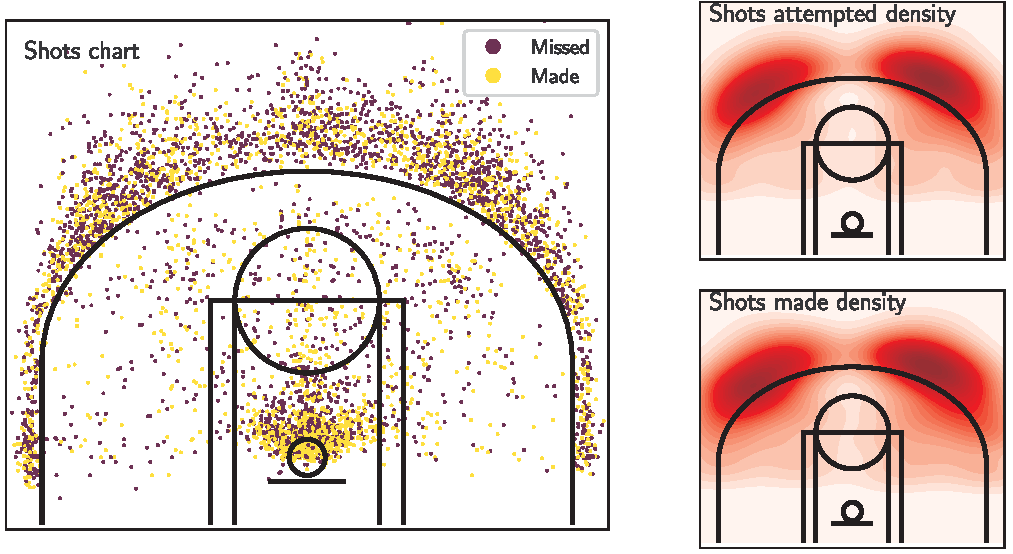
\includegraphics[width=\textwidth]{curry}
    \caption{Made/Missed shots chart (left) and the estimated densities (right) for Stephen Curry.}
    \label{fig:shoots_make_miss}
\end{figure}


We estimate the functional principal components using the \texttt{Gram}, \texttt{(Tensor) PCA} and \texttt{2D/1D B-Splines} methods. For the \texttt{Gram} method, we directly use the estimated densities to estimate the eigencomponents. For the \texttt{(Tensor) PCA} method, the estimation of the multivariate eigenimages is based on the univariate estimation of $30$ univariate eigenimages. The estimation of the (univariate) eigenimages is performed with the FCP-TPA where the smoothing parameters are chosen via cross-validation in $[10^{-5}, 10^5]$. For the \texttt{2D/1D B-splines} method, the two components are expanded in tensor products of $13 \times 13$ B-splines. We do not add a smoothing penalty in that case, as the smoothing step is performed in the kernel density estimation.

Figure~\ref{fig:eigenfunctions_gram} shows the estimated mean surfaces and eigenfunctions for the \texttt{Gram} method. The functional principal components, as a representation of the deviation from the mean surface function, may take negative values, while densities can only take positive values. For presentation purposes, the functional principal components have been normalized between $-1$ and $1$. Blue areas correspond to negative values of the functional components, and thus contribute negatively to the density, while red area corresponds to positive values of the functional components, and thus contribute positively to the density. The decomposition of the density of made shots is similar that of attempted shots. The obtained functional components can be explained as different shooting behavior. The first component, accounting for $56.9\%$ of the variance explained, contrasts two-point and three-point shooting. A player with a positive score for $\phi_1$ will tend to take/attempt shots more behind the three-point line, while if he has a negative score, he will prefer shooting within the two-points zone. For the second component ($11.5\%$ of the variance explained), the contrast is between the left and right sides of the court. Similarly, if a player has a positive (resp. negative) score for $\phi_2$, he will prefer to shoot on the right (resp. left) side of the court while looking at the hoop. The third component ($9.4\%$ of the variance explained) contrasts shooting from the wing with shooting in the axis of the hoop. Positive (resp. negative) score players will shot in the axis of the hoop (resp. from the wing). The fourth component ($4.7\%$ of the variance explained) is more difficult to explain from a shooting behavior perspective. It may be linked to players having a preferred shooting location so that most of their shots are taken from the same position. The estimation of the eigencomponents with the \texttt{(Tensor) PCA} and \texttt{2D/1D B-Splines} methods are similar to the results with the \texttt{Gram} method and are thus provided in the Appendix \ref{sec:more_results}. 
\begin{figure}
    \centering
    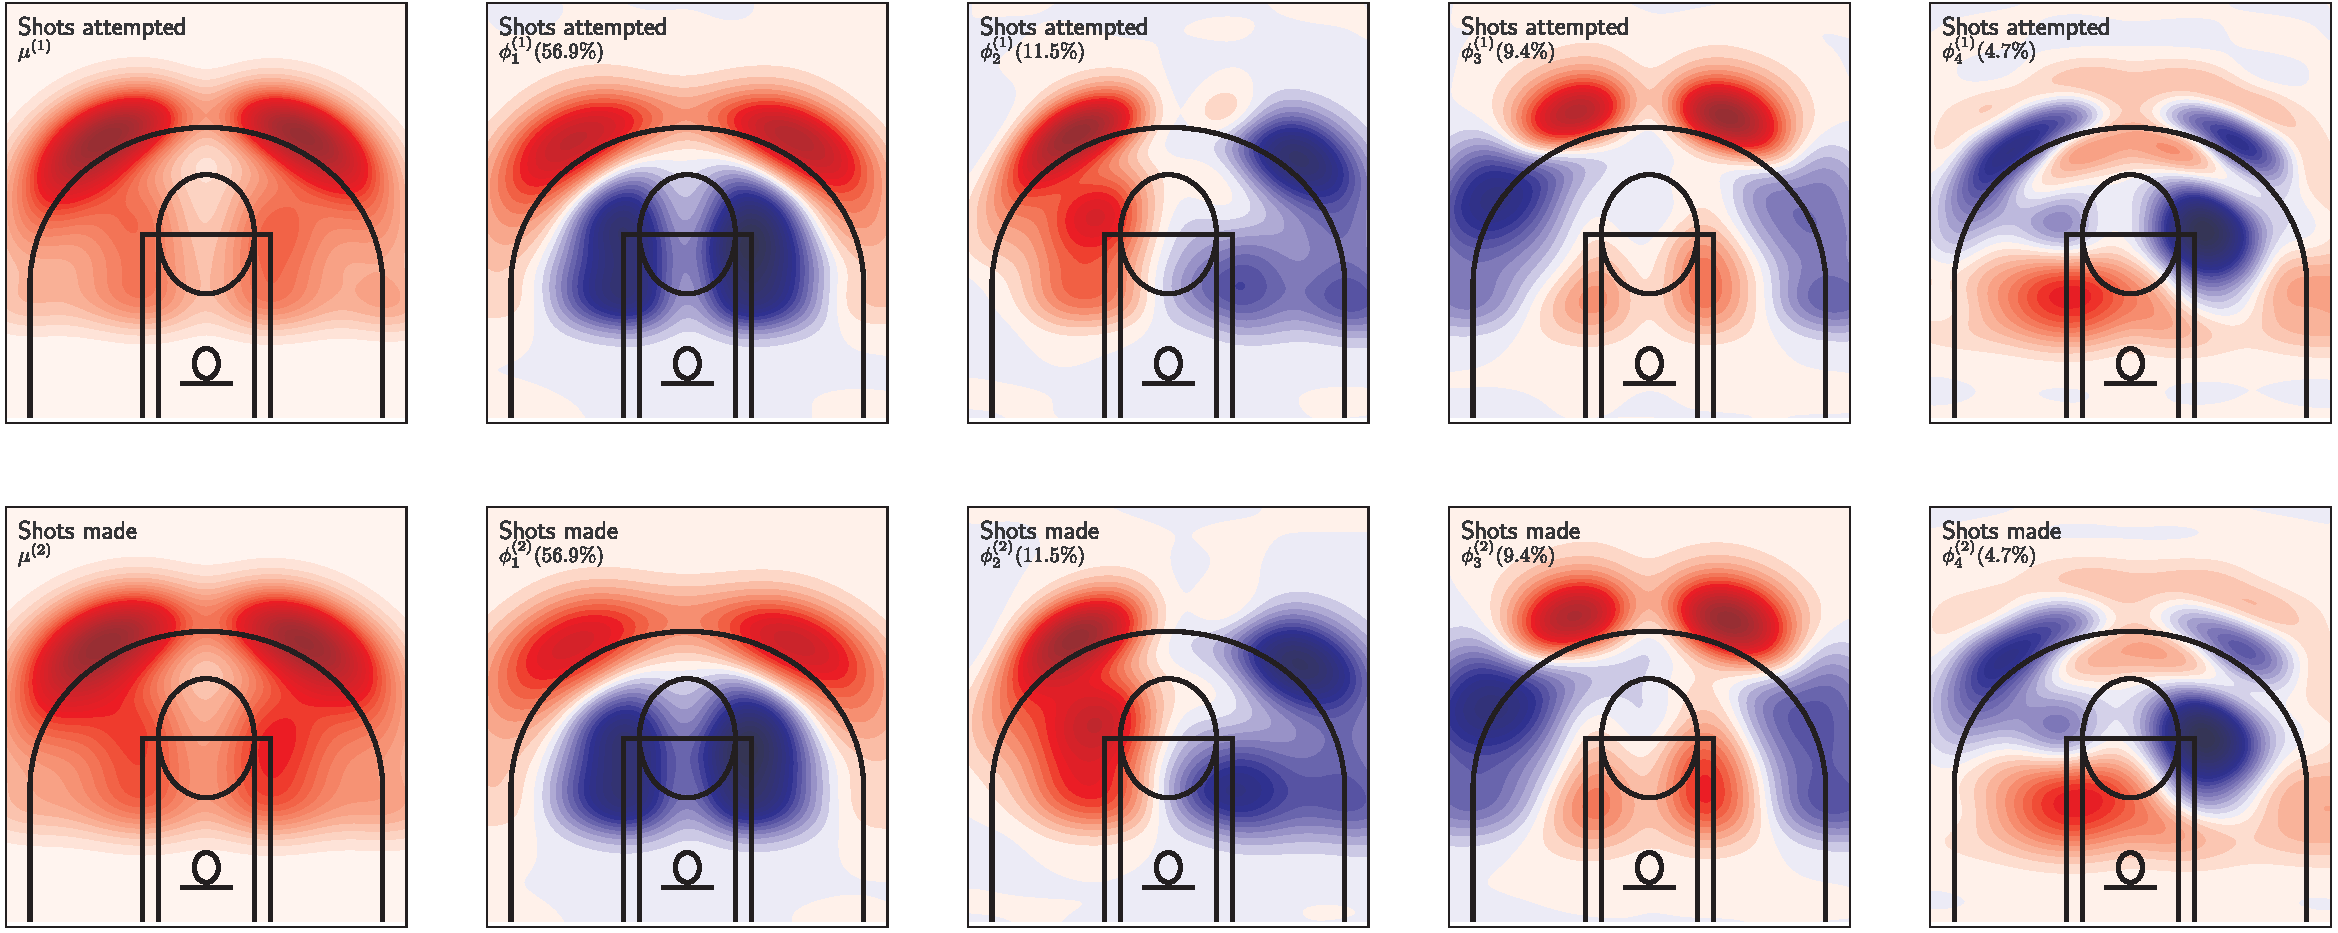
\includegraphics[width=\textwidth]{eigenfunctions_gram}
    \caption{The estimated mean surfaces (first column) and the estimated eigenfunctions (second to fifth columns) for the shots dataset using the \texttt{Gram} method.}
    \label{fig:eigenfunctions_gram}
\end{figure}
% section application (end)


% REFERENCES ---------
\bibliographystyle{apalike}
\bibliography{biblio}

\makeatletter\@input{ms_ref.tex}\makeatother
\end{document}

